% status: 0
% chapter: TBD

\title{Runtime comparasion of application between containorized vs standalone.}

\author{Anubhav Lavania}
\affiliation{%
  \institution{Indiana University}
  \streetaddress{Smith Research Center}
  \city{Bloomington} 
  \state{IN} 
  \postcode{47408}
  \country{USA}}
\email{anubhav.lavania@gmail.com}


% The default list of authors is too long for headers}
\renewcommand{\shortauthors}{G. v. Laszewski}


\begin{abstract}
Docker swarm enables clustering of numerous docker nodes to act as
single virtual machine. It enables clustering and scheduling of
different docker containers. 
Oracle Virtual box enables running guest operaing system on top of
base operating system and needs dedicated resources of underlying
hardware.
In this paper we will comare the performance of an application when
run on Docker swarm and Oracle VM.

\end{abstract}

\keywords{hid-sp18-413, Docker Swarm}


\maketitle


\section{Introduction}

This paper provides a comparasion of running an application in a
containerized environment vs running the same applicatin on a
standalone hardware. We will run an application on a docker swarm
cluster~\cite{hid-sp18-413-dockerswarm} of three raspberry pi's and
run the same aplication on a Ubuntu VM run using Oracle Virtual box and compare the performance.

The setup is shown in Figure~\ref{F:setup}.

\begin{figure}[!ht]
<<<<<<< HEAD
  \centering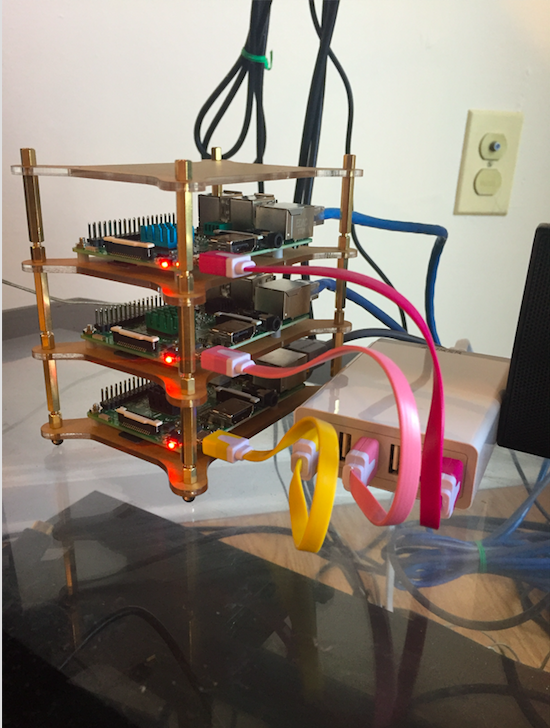
\includegraphics[width=\columnwidth]{images/hid-sp18-413-my3pi.png}
  \caption{3pihomesetup}
=======
  \centering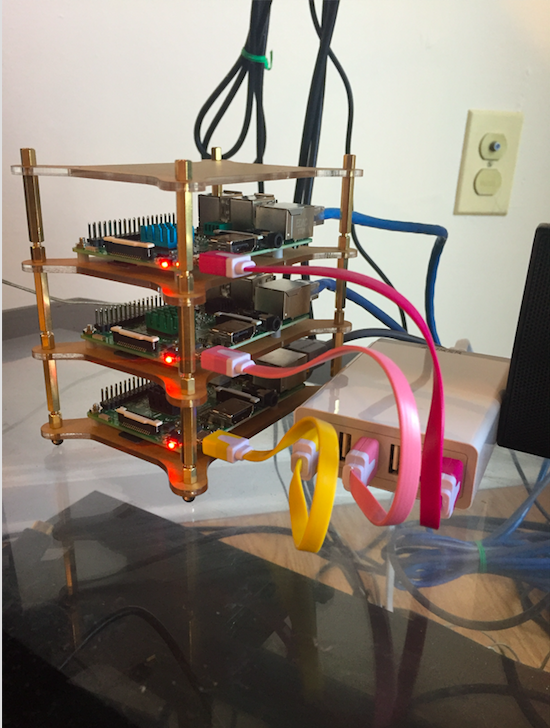
\includegraphics[width=\columnwidth]{images/hid-sp18-413-my3pi.jpeg}
  \caption{my3pihomesetup}\label{F:setup}
>>>>>>> 6fee30260492cb23d55b49cb03428dec64cc528c
\end{figure}


\begin{acks}

  The authors would like to thank Dr.~Gregor~von~Laszewski for his
  support and suggestions to write this paper.

\end{acks}

\bibliographystyle{ACM-Reference-Format}
\bibliography{report} 

